\chapter{Основы}

\section{Ваше тело~--- просто кипа еды}
\begin{quote}
\textit{``То, что вы называете <<моим телом>>~--- это просто накопление пищи, которую вы едите. Итак, какая пища вы едите, должна зависеть не от ваших ценностей и этики или от того, что вы думаете об этом, а от того, чего хочет организм. Пища~--- это о теле. Если вы достаточно хорошо знаете, если вы просто прикоснетесь к какому-нибудь кусочку пищи, вы узнаете, как эта пища будет вести себя в вашем организме.
\\[3pt]
Когда речь идет о еде, спросите организм, какая еда ему действительно нравится. Попробуйте разные виды пищи и посмотрите, каково ваше тело после еды. Если ваше тело чувствует себя очень подвижным, энергичным и приятным --- оно счастливо. Если организм чувствует себя вялым и нуждается в накачке кофеином или никотином, чтобы не спать~--- он не счастлив.
\\[3pt]
Питаться разумно~--- значит понимать и снабжать организм тем топливом, на которое он рассчитан, чтобы он мог функционировать наилучшим образом. От того, как вы едите, зависит не только ваше физическое здоровье, но и то, как вы думаете, чувствуете и ощущаете жизнь.
\\[3pt]
Прежде всего, пища, которую вы едите~--- это жизнь. Другие формы жизни отказываются от своей жизни, чтобы поддержать нас. Если вы едите с огромной благодарностью за все живые существа, которые отказываются от своей жизни, чтобы поддерживать свою жизнь, пища будет вести себя внутри вас совсем по-другому.''
\\[5pt]
\rightline{\textbf{--- Садхгуру}}}
\end{quote}

\section{Вегетарианство или невегетарианство}
\begin{itemize}
\item Для различных видов деятельности необходимо другое тело.
\item Лучше всего, чтобы люди питались в соответствии с характером их деятельности.
\item Для видов деятельности, которыми в настоящее время занимается большинство людей, вегетарианская пища лучше для системы, чем невегетарианская пища.
\item Если необходимо есть невегетарианскую пищу, то лучше всего будет рыбу. Она легко усваивается и имеет очень высокую пищевую ценность.
\end{itemize}




\begin{DidYouKnow}
\begin{wrapfigure}{r}{0.6\textwidth}
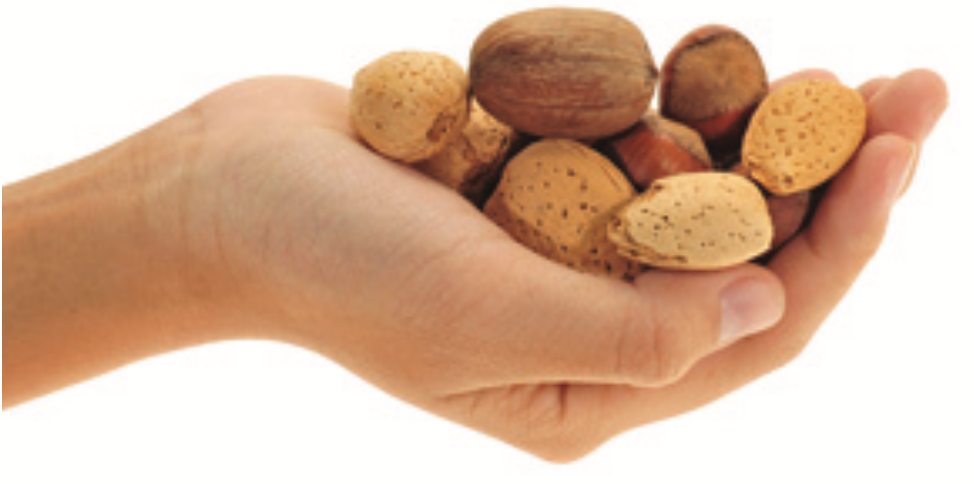
\includegraphics[width=0.5\textwidth]{img/hand.png}
    \caption{\textit{Богатые белками растительные продукты дают дополнительные преимущества, которых нет в мясе. Некоторые растительные продукты включают защитные фитохимические вещества, такие как изофлавоны в сое. Фасоль же содержит белок в сочетании с волокнами, которые выравнивают уровень сахара в крови.}}
\end{wrapfigure}

Мясо~--- богатый источник белка. Но важно отметить, что в нашем ежедневном рационе питания требуется всего несколько граммов белка, а избыточное потребление белка может вызвать рак \cite{ProteinCancer} и другие проблемы со здоровьем \cite{ProteinKidney}. Пророщенные граммы, орехи, фрукты и сухофрукты являются хорошими источниками белка, которые могут удовлетворить все потребности вашего организма. Потребление орехов также уменьшает риск сердечной болезни. \cite{NutsForTheHeart}
\end{DidYouKnow}

\section{Как много нужно съесть}
Исследования показали, что человеческий мозг работает лучше всего, когда желудок пуст. Исследователи обнаружили, что пустой желудок вырабатывает грелин, гормон, который несет в мозг сообщение о том, что желудок голоден. Интересно, что этот гормон выполняет и другие функции. Грелин стимулирует и повышает работоспособность гиппокампа, области в мозге, которая отвечает за обучение, память и пространственный анализ \cite{EmptyStomachIntelligence}, держит нас в внимательными, активными и сосредоточенными.  Это, конечно, не означает, что мы никогда не должны есть, а скорее указывает на то, что мы должны осознавать, сколько мы едим.

Садхгуру подробно рассказывает о том, как мы можем извлечь максимум пользы в течении дня, оптимизируя потребление пищи.

\begin{quote}
\textit{``Не стоит есть весь день. Если вам меньше тридцати лет, трехразовое питание прекрасно впишется в вашу жизнь. Если вам больше тридцати лет, то лучше сократить его до двухразового питания. Наше тело и мозг работают в полную силу только тогда, когда желудок пуст. Будьте осознанными и ешьте так, чтобы в течение двух с половиной часов пища выходила из желудка, а в течение двенадцати-восемнадцати часов она полностью выходила из организма. Если вы будете поддерживать это простое понимание, вы будете испытывать гораздо больше энергии, ловкости и бодрости. Это ингредиенты успешной жизни, независимо от того, что вы решили делать.''
\\[5pt]
\rightline{\textbf{--- Садхгугру}}}
\end{quote}

\begin{figure}
    \centering
    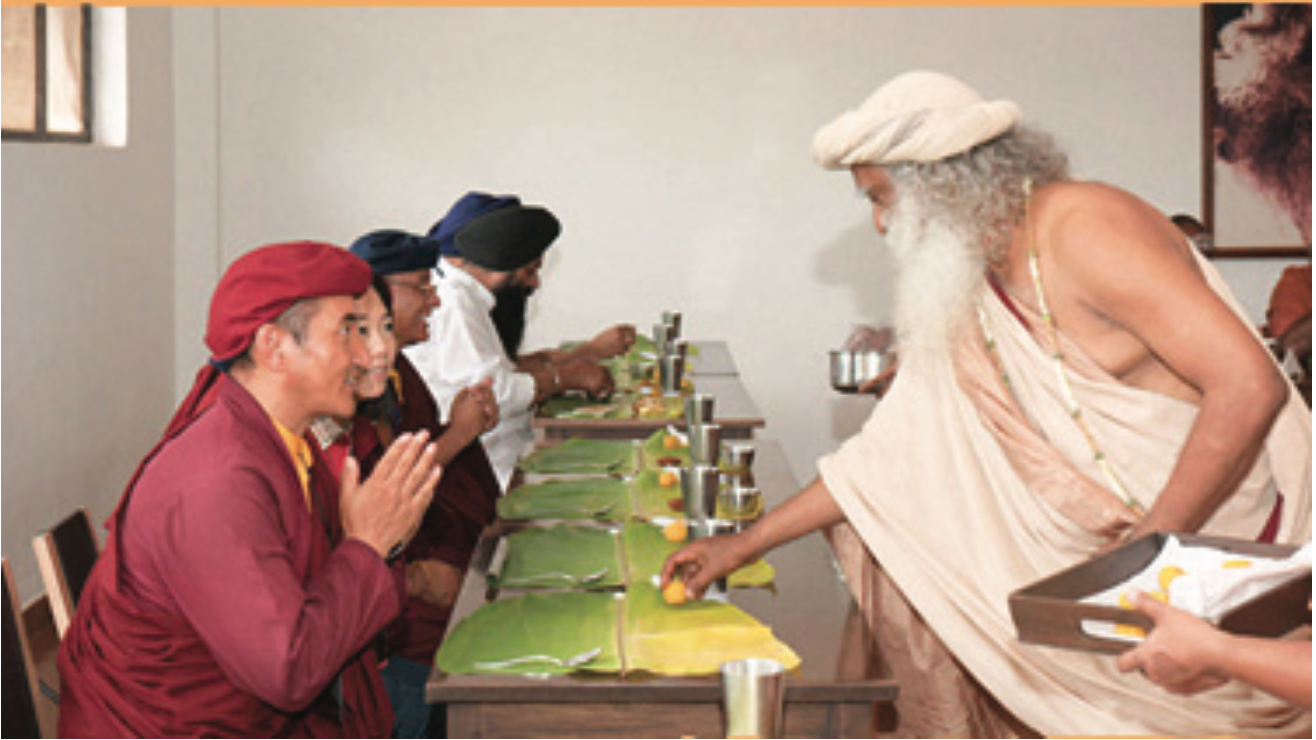
\includegraphics[width=\textwidth]{img/deligates.png}
\begin{quote}\small
\textit{``Истинная радость в еде~--- это осознание того, что другая жизнь готова слиться с вашей собственной жизнью и стать частью вас.''
\\[5pt]
\rightline{\textbf{--- Садхгугру}}}
\end{quote}
    \caption{Садхгуру служит делегатам \href{http://blog.ishafoundation.org/inside-isha/happenings/celebrations-of-the-14th-anniversary-of-dhyanalinga-consecration/}{Межрелигиозных Делибатов}, проходящих в \href{http://blog.ishafoundation.org/inside-isha/happenings/celebrations-of-the-14th-anniversary-of-dhyanalinga-consecration/}{Йога-центре Иша} 23 июня 2013 года.
    }

\end{figure}

\section{Приготовленные или сырые овощи}
\begin{itemize}
\item Не все ферменты, необходимые для пищеварительного процесса, присутствуют в организме. Пища, которую мы едим, также должна способствовать пищеварению.
\item Процесс приготовления пищи уничтожает значительную часть этих ферментов в пище.
\item Поедание пищи после этого процесса разрушения не дает такого же количества жизненной энергии системе. Организм с трудом восстанавливает эти разрушенные ферменты.
\item Поэкспериментируйте и посмотрите, если вы добавите в свой рацион сырую вегетарианскую пищу, то это позволит сохранить организм здоровым и энергичным. Начните с 25\% натуральной пищи и медленно доводите ее до 100\% в течение четырех-пяти дней. Продержитесь там в течение одного-двух дней и снова сократите долю за пять дней до 50\% натуральной пищи и 50\% готовой пищи. Это идеальная комбинация для большинства людей, которые желают быть активными шестнадцать-восемнадцать часов в день.
\item Естественная пища требует больше времени, чем приготовленная, потому что ее нужно больше жевать. Поэтому вам необходимо сознательно проводить больше времени за столом, чтобы убедиться в том, что вы съели достаточно еды.
\end{itemize}

\begin{KeepInMind}
При употреблении в пищу сырых продуктов обязательно замочите их в небольшом количестве соленой воды, а затем промойте в холодной воде. Это убьет все вредные организмы на пище.
\end{KeepInMind}

\section{Пережуйте это!}
\begin{itemize}
\item Правильное жевание пищи играет важную роль в пищеварении. Исследования показывают, что для крахмалистой пищи 40\% пищеварения должно происходить со слюной.
\item После еды дайте перерыв не менее двух часов перед сном. Пищеварение повышает вашу метаболическую активность. Если вы будете спать в таком состоянии, вы не будете ни хорошо спать, ни хорошо переваривать! В зависимости от того, что вы едите, до 80\% пищи может остаться непереваренной, если вы будете спать сразу после еды.
\item Фрукты следует есть за полтора-два часа до еды. Лучше всего употреблять фрукты во время сезона, выращенные в вашем населенном пункте.
\item  Избегайте пить воду во время еды. Пейте немного воды за несколько минут до еды или через тридцать - сорок минут после еды.
\end{itemize}

\begin{DidYouKnow}
Чрезмерное потребление воды может вызвать отёк мозга. Всегда лучше пить лишь немного больше, чем нужно для утоления жажды. Воду также можно оставить на ночь в медном сосуде. Это уничтожает бактерии и питает воду мощной энергией. Было обнаружено, что медные поверхности, протестированные в больничных отделениях интенсивной терапии (ICU), убивают 97\% бактерий, способных вызывать внутрибольничные инфекции \cite{CopperBacteria}.
\end{DidYouKnow}

Садхгуру подробно рассказывает об индийской традиции употребления различных продуктов в разное время года и о том, как эта практика помогает организму справляться с меняющейся погодой.

\begin{quote}
\textit{``В Индии, и особенно в Южной Индии, летом пища готовится одним способом, в сезон дождей --- еще одним, а зимой --- третим, в соответствии с имеющимися в то время овощами и тем, что подходит для организма. Хорошо привнести эту мудрость и питаться в соответствии с потребностями организма и в соответствии с погодой или климатом, в котором мы живем.
\\[3pt]
Например, зимой кожа обычно ломается, потому что климат становится холодным, а люди раньше не использовали крема или лосьоны. Есть определенные продукты, такие как кунжут и пшеница, которые производят тепло в организме. Поэтому, когда наступает декабрь, все едят кунжут ежедневно. Он сохраняет тепло тела и чистоту кожи. Если в теле много тепла, ваша кожа не сломается. Летом тело нагревается, поэтому ели охлаждающие продукты. Например, в Тамилнаде люди ели камбу (жемчужное просо). Рацион буллы устроен так, чтобы помочь организм приспособиться к текущему сезону.''
\\[5pt]
\rightline{\textbf{--- Садхгугру}}}
\end{quote}


\section{Смеси и сочетания}
В Индии еда и процесс принятия пищи были важным аспектом культуры. Какую еду и как ее есть~--- неотъемлемая часть повседневной жизни каждой семьи.


\begin{quote}
\textit{``Тело обладает феноменальным чувством памяти. Одна молекула ДНК в вашем теле несет в себе гораздо больше памяти, чем может запомнить весь ваш мозг. Ваша ДНК помнит, какой нос был у вашего прадеда, и помещает его вам на лицо. Существует определенный аспект кармы, называемый рунану бандха. Тело ведет учет всего, что произошло. Рунану бандха происходит, когда происходит определенное количество встреч и общения между людьми. Особенно в моменты близости с другим телом, бандха рунану гораздо глубже.
\\[3pt]
Другое дело~---тип пищи, которую вы едите. Всякий раз, когда приходит немного изобилия, люди думают, что они должны съесть все за один прием пищи. Если вы ходите на какие-либо богатые обеды~--- это становится безумием. Некоторое время назад я был на мероприятии, где кто-то очень гордо объявил, что у них есть 270 различных сортов пищи. Люди берут все понемногу и едят. Организм путается с такой пищей. Как только ваше тело запутается, вы сойдете с ума во многих отношениях. В Индии это понимание было всегда. Ортодоксальные люди никогда не ели больше двух-трех блюд за один прием пищи, и эти три блюда всегда сочетались друг с другом. Интеллект желудка таков, что помещение различных видов веществ в него не сочетается с естественным процессом.''
\\[5pt]
\rightline{\textbf{--- Садхгугру}}}
\end{quote}
